\documentclass{article}
\usepackage[T1]{fontenc}
\usepackage{hyperref}
\usepackage[utf8]{inputenc}
\usepackage[brazilian]{babel}
\usepackage{graphicx}
\usepackage[a4paper, total={6in, 8in}]{geometry}

\graphicspath{ {./imagens/} }
\hypersetup{
    colorlinks=true,
    linkcolor=blue,
    filecolor=magenta,      
    urlcolor=cyan,
    pdftitle={Overleaf Example},
    pdfpagemode=FullScreen,
}

\selectlanguage{brazilian}

\title{Rede neural convolucional reconhecedora de raças de cachorro}
\author{Lucas S. Santos, Rafael N. Lourenço}
\date{Junho 2022}

\begin{document}

\maketitle
\newpage
\section{Teoria}
Uma rede neural convolucional é uma arquitetura que utiliza de técnicas para reconhecer padrões, muito usada para criar modelos que reconhecem imagens.
Esse algoritmo de aprendizado profundo contém três camadas principais que são:
\begin{itemize}
    \item Camada convolucional
    \item Camada de pooling
    \item Camada totalmente conectada
\end{itemize}

\section{Implementação}
O modelo usado é do modo sequencial, i,e. aplica as camadas em sequência. O padrão repetido três vezes foi a aplicação de Conv2d, MaxPooling2d, Dropout e após essas repetições foi aplicada uma camada de Flatten e Dense. O conjunto de dados utilizado foi o de \href{https://www.kaggle.com/competitions/dog-breed-identification/data}{raças de cachorros}.\\
Nesse conjunto de dados foi feito um tratamento nas imagens deixando elas em preto e branco e aplicando um filtro de Blur e finalizando com outro de SobelXY.\\\\
Esses foram alguns dos resultados:\\\\
\begin{figure}[h]
    \centering
    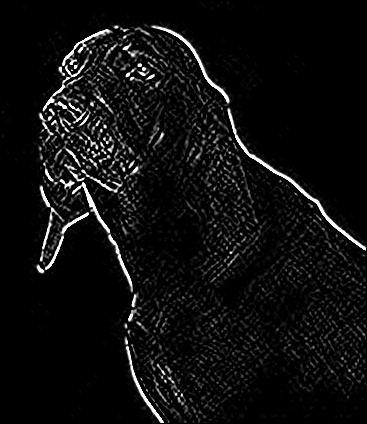
\includegraphics[scale=0.3]{ex_cachorro}
    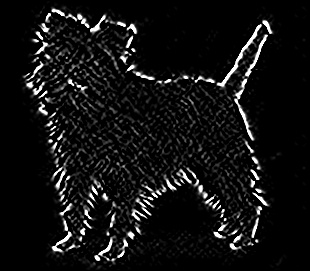
\includegraphics[scale=0.3]{ex_cachorro2}
    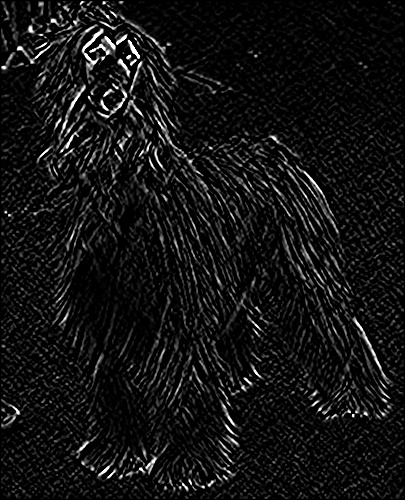
\includegraphics[scale=0.3]{ex_cachorro3}
    \caption{Imagens de cachorros com filtros Blur e SobelXY}
\end{figure}


\newpage

\section{Resultados}

Apesar de os resultados não serem ótimos houve um progresso em comparação com os modelos anteriores, além do que o conjunto de dados de raça de cachorro é bem complexo, pois possui muito ruído e nem em todas imagens tem o contorno do animal, a variedade de cores nas imagens e falta de padrão no sentido de estar centralizado dificultou muito o aprendizado.

\begin{figure}[h]
    \centering
    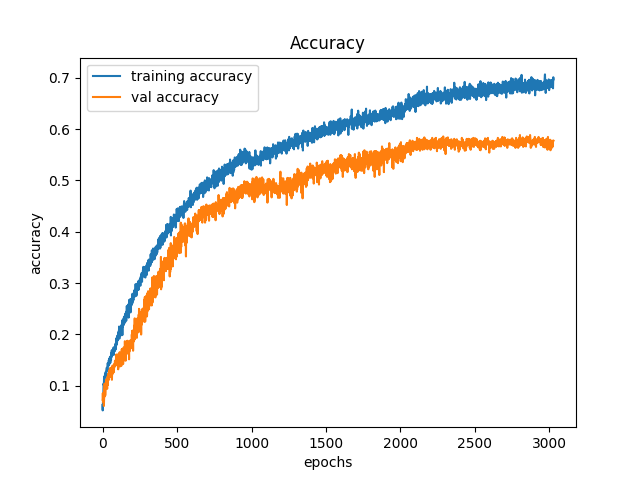
\includegraphics[scale=0.45]{longo_epochs_accuracy_old}
    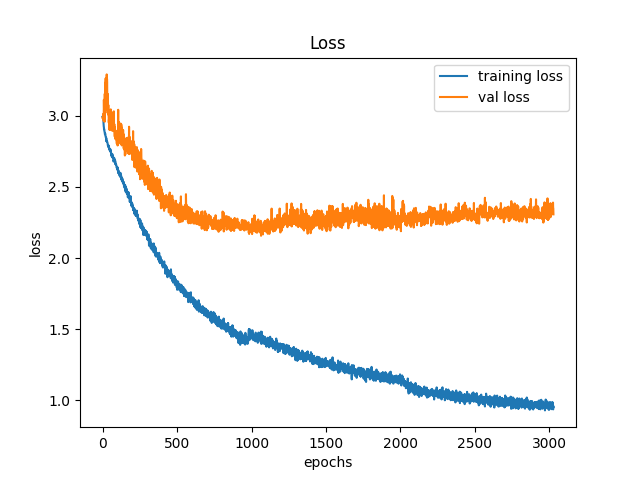
\includegraphics[scale=0.45]{longo_epochs_loss_old}
    \caption{Modelo antigo}
\end{figure}

Ambos os modelos tiveram sua acurácia abaixo de 0.6, acreditamos que devido o seja devido ao conjunto de dados, foram feitos diversos modelos, e somente esses dois chegaram a um resultado relevante.
\\
No último modelo após mais de 700 épocas foram adicionadas, mais algumas imagens tiradas da internet, parecendo ter uma melhora significativa na acurácia, houve também a remoção de algumas outras imagens do conjunto, como o caso dos filhotes.

\begin{figure}[h]
    \centering
    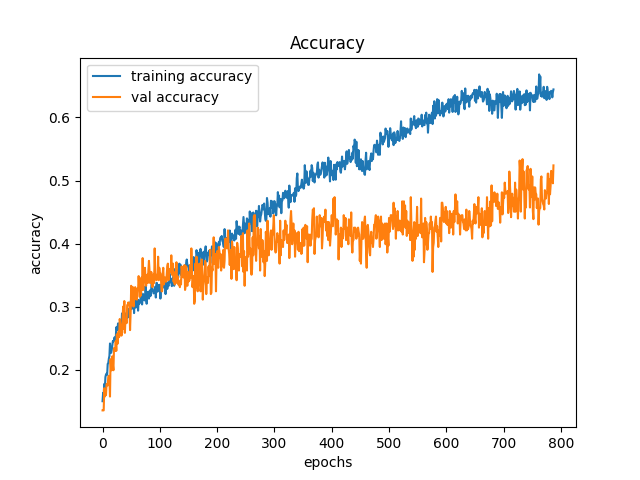
\includegraphics[scale=0.45]{longo_epochs_accuracy}
    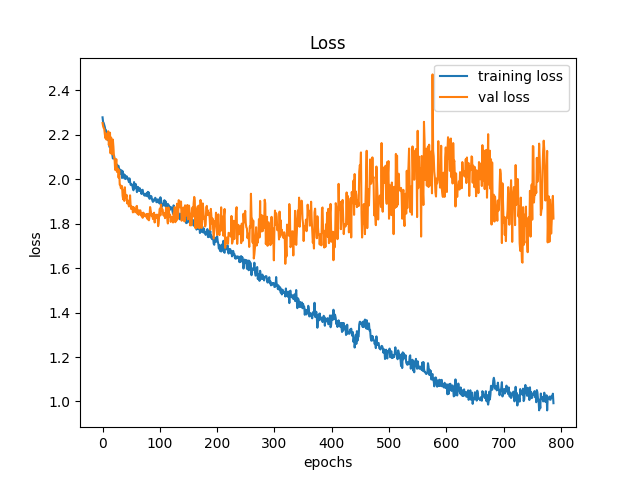
\includegraphics[scale=0.45]{longo_epochs_loss}
    \caption{Modelo novo}
\end{figure}

\section{Referencias}
\href{https://crivelaro.notion.site/Bot-de-Discord-de-Classifica-o-de-Imagens-com-Deep-Learning-498ca37d41c549fb90c403f8ccf3804e}{Bot de Discord de Classificação de Imagens com Deep Learning}\\
\href{https://www.youtube.com/watch?v=dFdMyUbtKM4}{Image classification from scratch - Keras Code Examples}\\
\href{https://keras.io/examples/vision/image_classification_from_scratch/}{Image classification from scratch}\\
\href{https://curiousily.com/posts/hackers-guide-to-fixing-underfitting-and-overfitting-models/}{Hacker's Guide to Fixing Underfitting and Overfitting Models}\\
\href{https://devcenter.heroku.com/articles/build-docker-images-heroku-yml}{Building Docker Images with heroku.yml}\\
\href{https://wavesofvoqueric.com/software/2020/03/31/19/29/opencv-image-to-tensorflow-tensor/}{OpenCV Image to TensorFlow Tensor}\\
\href{https://data-flair.training/blogs/python-project-traffic-signs-recognition/}{Python Project on Traffic Signs Recognition with 95\% Accuracy using CNN \& Keras}\\
\href{https://www.youtube.com/watch?v=pAhPiF3yiXI}{TensorFlow Tutorial 3 - Neural Networks with Sequential and Functional API}\\
\href{https://www.youtube.com/watch?v=IubEtS2JAiY&list=PLZbbT5o_s2xrwRnXk_yCPtnqqo4_u2YGL&index=2}{TensorFlow and Keras GPU Support - CUDA GPU Setup}\\
\href{https://www.youtube.com/watch?v=FK77zZxaBoI}{Layers in a Neural Network explained}\\
\href{https://www.youtube.com/watch?v=YRhxdVk_sIs}{Convolutional Neural Networks (CNNs) explained}\\
\href{https://www.youtube.com/watch?v=83LYR-1IcjA}{Neural Networks Pt. 4: Multiple Inputs and Outputs}\\
\href{https://keras.io/guides/functional_api/}{The Functional API}\\
\href{https://www.deeplearningbook.com.br/introducao-as-redes-neurais-convolucionais/}{Capítulo 40 – Introdução as Redes Neurais Convolucionais}\\
\end{document}
